\documentclass[11pt,a5paper]{article}

\usepackage[T1]{fontenc} % font encoding, lubab õ tähte kasutada
\usepackage[utf8]{inputenc} % oleme siiski 21. sajandis, vajadusel on ka olemas utf8x
\usepackage{lmodern, microtype} % lmodern ja micrtype käivad käsikäes, teeb teksti ilusamaks
\usepackage{enumerate}
\usepackage{caption}
\usepackage[estonian]{babel} % eesti keele poolitamisreeglid jpm
\usepackage[per = fraction, expproduct=cdot, decimalsymbol=comma]{siunitx} % https://www.texlive.info/CTAN/macros/latex/contrib/siunitx/siunitx.pdf
\usepackage{graphicx}
\usepackage[european]{circuitikz}
\usepackage{wrapfig}
\usepackage{tikz}
\usepackage{pgfplots}
\usetikzlibrary{decorations.pathreplacing, positioning}
\usetikzlibrary{arrows,calc,decorations.markings,math,arrows.meta}
\usepackage{epstopdf} %minul on vaja, et .eps pilte saada
\usepackage{float}
\usepackage{amsmath}
\usepackage{hyperref} %linkide jaoks jaluses
%paneme kõik mõõdud paika
\topmargin=-2.5cm \textheight=18cm \textwidth=12.77cm
\oddsidemargin=-1.5cm  \evensidemargin=-1.5cm
\setlength{\parindent}{0pt} \setlength{\parskip}{6pt} \sloppy
\relpenalty=10000 \binoppenalty=10000 % Tekstisisestes valemites reavahetusi ärgu olgu
\pagestyle{empty} % ilma leheküljenumbrita
\newcommand{\numb}[1]{\vspace{5pt}\textbf{\large #1}}
\newcommand{\nimi}[1]{(\textsl{\small #1})}
\newcommand{\punktid}[1]{(\emph{#1~p.})}
\newcommand{\autor}[1]{}
%\newcommand{\autor}[1]{\emph{ Autor: #1}} Temporarily surpressed
\newcounter{ylesanne}
\newcommand{\yl}[1]{\addtocounter{ylesanne}{1}\numb{\theylesanne.} \nimi{#1} \newblock{}}


\begin{document}

\begin{center}
	\textbf{\Large Eesti koolinoorte 68. füüsikaolümpiaad} \par
	\emph{6. veebruar 2021. a. \\Gümnaasiumi ülesanded (10.-12. klass)}
\end{center}
\resizebox{\textwidth}{!}{%
	\emph{%
		\begin{tabular}{@{}l@{}}
			Lahendamisaeg on 5 tundi. \\
			Iga osavõtja võib lahendada kõiki pakutud ülesandeid. \\
			Arvesse lähevad 5 suurima punktide arvu saanud teoreetilist ja 1 eksperimentaalne ülesanne. \\
			Kasutada võib kirjutus- ja joonestusvahendeid ning kalkulaatorit. Muud abivahendid on keelatud.\\
			Eksperimentaalülesande lahendamisel võib kasutada üksnes loetelus toodud vahendeid. \\
			Mõõtemääramatuse hindamist ei nõuta.
		\end{tabular}
	}
} \par

\yl{KUUL SFÄÄRIS}
Kausis, mille sisekülje pinnaks on poolsfäär raadiusega $R=\SI{50}{\centi\meter}$, veereb ühtlase kiirusega mööda horisontaaltasapinnalist ringjoont kuulike. Kuuli tiirlemistasandi kõrgus kausi põhjast on $h=\SI{10}{\centi\meter}$. Leidke kuuli tiirlemisperiood. Eeldage, et kuuli läbimõõt on kausi raadiusega võrreldes tühine ning hõõrdetegur kuuli ning kausi vahel on samuti tühiselt väike. Gravitatsioonikiirendus on $g=\SI{9.8}{\meter\per\second\squared}$.
\punktid{8} \autor{Markus Rene Pae}

\yl{KLAASPUDEL}
Klaaspudel ruumalaga $V_0=\SI{1}{\liter}$ on osaliselt täidetud veega, mis on temperatuuril $T_0=\SI{20}{\celsius}$. Algul on pudelis olev rõhk võrdne välise rõhuga, mis on $p_0=\SI{100}{\kilo\pascal}$. Pudel suletakse ja pannakse sügavkülma nii, et seal olev vesi hakkab jäätuma. Pudel kannatab maksimaalset ülerõhku $\Delta p=\SI{300}{\kilo\pascal}$. Leidke maksimaalne kogus vett $V_{\text{v}}$, mis võis alguses pudelis olla, et pudel ei läheks vee jäätumisel katki. Vee tihedus lugeda kõikidel temperatuuridel võrdseks $\rho_{\text{v}}=\SI{1000}{\kilo\gram\per\meter\cubed}$ ja jää tihedus on $\rho_{\text{j}}=\SI{920}{\kilo\gram\per\meter\cubed}$. Eeldage, et pudelis olev õhk ja vesi on soojuslikus tasakaalus terve protsessi vältel ja et juurde tekkiv jää saab vabalt liikuda pudeli õhuga täidetud osasse.

\emph{Vihje.} Pudelis olevat õhku võib käsitleda kui ideaalset gaasi, mille rõhk $p$, ruumala $V$ ja absoluutne temperatuur $T$ (mida SI süsteemis mõõdetakse kelvinites) rahuldavad seost $\tfrac{pV}{T}=\textit{const}$.
\punktid{8} \autor{Kaur Aare Saar}

\yl{JOOGID}
Kauril on 3 anumat, igas neist on võrdselt $\SI{1}{\kilo\gram}$ vett. Anumates oleva vee temperatuurid on vastavalt $\SI{10}{\celsius}$, $\SI{20}{\celsius}$ ja $\SI{30}{\celsius}$.
% Lisaks on Kauril mõõdukann ja palju anumaid.
Kas Kauril on võimalik vaid antud vedelikke segades \\
\osa teha $2$ jooki, kumbki massiga $\SI{1.5}{\kilo\gram}$ ja temperatuuridega vastavalt $\SI{13}{\celsius}$~ja~$\SI{27}{\celsius}$;\\
\osa teha $5$ jooki, igaüks massiga $\SI{0.5}{\kilo\gram}$ ja temperatuuridega vastavalt $\SI{12}{\celsius}$,~$\SI{17}{\celsius}$,~$\SI{18}{\celsius}$,~$\SI{20}{\celsius}$~ja~$\SI{22}{\celsius}$?\\
Eeldage mõlema puhul, et soojusvahetust keskkonnaga ei toimu.
\punktid{8} \autor{Kaarel Hänni}


\yl{BATÜSKAAF}
Monika sõidab keset ookeanit batüskaafi ehk süvaveeliikuriga. Ühel hetkel
ütlesid üles batüskaafi mootorid, millega veepaakidest vett välja pumbata. See
vajus $h=\SI{10}{\kilo\meter}$ sügavusele ookeani põhja ja jäi sinna lebama.
Selleks, et batüskaaf pinna poole tõusma hakkaks, on selle paakidest vaja ookeanisse
välja pumbata $V=\SI{1}{\liter}$ vett, mille tulemusena jääb paakidesse vaakum.
Monikal on võimalik kasutada $d=\SI{1}{\centi\meter}$ läbimõõduga silindrilist
pumpa ja erinevaid lihtmehhanisme selle pumbaga töötamiseks. Kui kaua kulub Monikal
vee välja pumpamiseks aega, kui ta suudab rakendada jõudu $F=\SI{500}{\newton}$
ja teha tööd keskmise võimsusega $P=\SI{100}{\watt}$. Ookeani tihedus on
$\rho=\SI{1030}{\kilo\gram\per\meter\cubed}$ ning gravitatsioonikiirendus
$g=\SI{9.8}{\meter\per\second\squared}$. Õhurõhku võib ignoreerida.
\punktid{8} \autor{Kaido Reivelt}

\yl{VOOLUALLIKAS}
Elektriskeem koosneb vooluallikast, mis annab välja konstantset voolu $I_0$ ja sellega rööpselt ühendatud sisetakistusest $R$. Leidke maksimaalne võimsus, mis saab klemmide $A$ ja $B$ vahele ühendatud tarbijal eralduda.
\punktid{8} \autor{Jaan Toots}
\begin{figure}[H]
  \centering
  \begin{circuitikz} \draw
    (0,0) to[I=$I_0$] (0,2)
    to[short] (2,2)
    to[R,l=$R$] (2,0)
    to[short] (0,0)

    (2,2) to[short, -o] (4,2)node[right]{$A$}
    (2,0) to[short, -o] (4,0)node[right]{$B$}
    % (3.3,2) to[open, v^=$V$] (3.3,0)
    ;
  \end{circuitikz}
\end{figure}

\yl{JALGRATTUR}
Samal ajal, kui jalgrattur sõidab mööda kindlat teelõiku, alustab auto juhuslikul ajahetkel juhuslikust kohast sellel teelõigul sõitu. Auto sõidab jalgratturiga samas suunas, kuid kaks korda kiiremini, ning mõlemad sõidavad teelõigu lõpuni. Mis on tõenäosus, et auto sõidab jalgratturist mööda?
\punktid{10} \autor{Jarl Patrick Paide}

\yl{RIPPUV LAENG}
Punktlaeng $q_1$ ripub lakke kinnitatud nööri otsas, mille pikkus on $L$. Teine samamärgiline punktlaeng $q_2$ on nöörist sõltumatult fikseeritud täpselt nööri kinnituskoha alla kaugusele $2h$ laest. Leidke milline peab olema esimese punktlaengu mass, et selle kaugus laest oleks $h$.
\punktid{10} \autor{Kaur Aare Saar}

\newpage
\begin{wrapfigure}{r}{0.45\textwidth}
  \begin{center}
		\vspace{-15pt}
		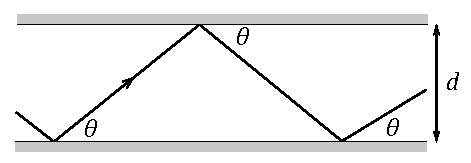
\includegraphics[width=0.47\textwidth]{lainejuht_yl.pdf}
		\vspace{-35pt}
  \end{center}
\end{wrapfigure}
\yl{LAINEJUHT}
Optilise telekommunikatsiooni arengu algusaegadel pakuti üheks lahenduseks signaali edastamiseks lainejuhti, kus valgus levib edasi ruudukujulise ristlõikega õõnsuses, mille sisemine pind on kaetud peegeldava pinnaga. Sellises lainejuhis levib valgus ainult diskreetsete nurkade $\theta$ korral (vt joonis), mille jaoks saab lihtsustatult kirjutada seose $\sin\theta=\tfrac{\lambda N}{2d}$, kus $\lambda$ on valguse lainepikkus, $d$ on lainejuhi läbimõõt ning $N=1,2,\dots$ on positiivne täisarv.

Alloleval graafikul on toodud ühe taolise lainejuhi läbipaistvuse sõltuvust nurgast $\theta$, kui seda läbib valgus lainepikkusega $\SI{1.55}{\micro\m}$. Leidke, kui kaugele on võimalik selle lainejuhiga optilist signaali saata nii, et selle intensiivsus ei väheneks rohkem kui $10$ korda, kui lainejuhi sisemust katva peegeldava pinna peegeldustegur on $R=99.8\%$ (st peegeldub $99.8\%$ valgusest).
\punktid{10} \autor{Hans Daniel Kaimre}

\begin{figure}[H]
	\centering
	\begin{tikzpicture}
\begin{axis}[
    width=0.9\textwidth,
    height=3.5cm,
    xlabel={$\theta$ ($^\circ$)},
    ylabel={Läbipaistvustegur},
    xmin=0, xmax=6,
    ymin=0, ymax=1.1,
    xtick={0,1,2,3,4,5,6},
    ytick={0,1},
    minor x tick num=9,
    grid=both,
    minor grid style={very thin,gray},
    major x grid style={black},
    major y grid style={very thin,gray},
]

\addplot[color=black,thick]
  coordinates {
  (0.1000,0)
  (0.1050,0)
  (0.1100,0)
  (0.1150,0)
  (0.1200,0)
  (0.1250,0)
  (0.1300,0)
  (0.1350,0)
  (0.1400,0)
  (0.1450,0)
  (0.1500,0)
  (0.1550,0)
  (0.1600,0)
  (0.1650,0)
  (0.1700,0)
  (0.1750,0)
  (0.1800,0)
  (0.1850,0)
  (0.1900,0)
  (0.1950,0)
  (0.2000,0)
  (0.2050,0)
  (0.2100,0)
  (0.2150,0)
  (0.2200,0)
  (0.2250,0)
  (0.2300,0)
  (0.2350,0)
  (0.2400,0)
  (0.2450,0)
  (0.2500,0)
  (0.2550,0)
  (0.2600,0)
  (0.2650,0)
  (0.2700,0)
  (0.2750,0)
  (0.2800,0)
  (0.2850,0)
  (0.2900,0)
  (0.2950,0)
  (0.3000,0)
  (0.3050,0)
  (0.3100,0)
  (0.3150,0)
  (0.3200,0)
  (0.3250,0)
  (0.3300,0)
  (0.3350,0)
  (0.3400,0)
  (0.3450,0)
  (0.3500,0)
  (0.3550,0)
  (0.3600,0)
  (0.3650,0)
  (0.3700,0)
  (0.3750,0)
  (0.3800,0)
  (0.3850,0)
  (0.3900,0)
  (0.3950,0)
  (0.4000,0)
  (0.4050,0)
  (0.4100,0)
  (0.4150,0)
  (0.4200,0)
  (0.4250,0)
  (0.4300,0)
  (0.4350,0)
  (0.4400,0)
  (0.4450,0)
  (0.4500,0)
  (0.4550,0)
  (0.4600,0)
  (0.4650,0)
  (0.4700,0)
  (0.4750,0)
  (0.4800,0)
  (0.4850,0)
  (0.4900,0)
  (0.4950,0)
  (0.5000,0)
  (0.5050,0)
  (0.5100,0)
  (0.5150,0)
  (0.5200,0)
  (0.5250,0)
  (0.5300,0)
  (0.5350,0)
  (0.5400,0.0000)
  (0.5450,0.0000)
  (0.5500,0.0000)
  (0.5550,0.0000)
  (0.5600,0.0000)
  (0.5650,0.0000)
  (0.5700,0.0000)
  (0.5750,0.0000)
  (0.5800,0.0000)
  (0.5850,0.0000)
  (0.5900,0.0000)
  (0.5950,0.0000)
  (0.6000,0.0000)
  (0.6050,0.0000)
  (0.6100,0.0000)
  (0.6150,0.0000)
  (0.6200,0.0000)
  (0.6250,0.0000)
  (0.6300,0.0000)
  (0.6350,0.0000)
  (0.6400,0.0000)
  (0.6450,0.0000)
  (0.6500,0.0000)
  (0.6550,0.0000)
  (0.6600,0.0000)
  (0.6650,0.0000)
  (0.6700,0.0000)
  (0.6750,0.0000)
  (0.6800,0.0000)
  (0.6850,0.0000)
  (0.6900,0.0000)
  (0.6950,0.0000)
  (0.7000,0.0000)
  (0.7050,0.0000)
  (0.7100,0.0000)
  (0.7150,0.0000)
  (0.7200,0.0000)
  (0.7250,0.0000)
  (0.7300,0.0000)
  (0.7350,0.0000)
  (0.7400,0.0000)
  (0.7450,0.0000)
  (0.7500,0.0000)
  (0.7550,0.0000)
  (0.7600,0.0000)
  (0.7650,0.0000)
  (0.7700,0.0000)
  (0.7750,0.0000)
  (0.7800,0.0000)
  (0.7850,0.0000)
  (0.7900,0.0000)
  (0.7950,0.0000)
  (0.8000,0.0000)
  (0.8050,0.0000)
  (0.8100,0.0000)
  (0.8150,0.0000)
  (0.8200,0.0000)
  (0.8250,0.0000)
  (0.8300,0.0000)
  (0.8350,0.0000)
  (0.8400,0.0000)
  (0.8450,0.0000)
  (0.8500,0.0000)
  (0.8550,0.0000)
  (0.8600,0.0000)
  (0.8650,0.0000)
  (0.8700,0.0000)
  (0.8750,0.0000)
  (0.8800,0.0000)
  (0.8850,0.0000)
  (0.8900,0.0000)
  (0.8950,0.0000)
  (0.9000,0.0000)
  (0.9050,0.0000)
  (0.9100,0.0000)
  (0.9150,0.0000)
  (0.9200,0.0000)
  (0.9250,0.0000)
  (0.9300,0.0000)
  (0.9350,0.0000)
  (0.9400,0.0000)
  (0.9450,0.0000)
  (0.9500,0.0000)
  (0.9550,0.0000)
  (0.9600,0.0000)
  (0.9650,0.0000)
  (0.9700,0.0000)
  (0.9750,0.0000)
  (0.9800,0.0000)
  (0.9850,0.0000)
  (0.9900,0.0000)
  (0.9950,0.0000)
  (1.0000,0.0000)
  (1.0050,0.0000)
  (1.0100,0.0000)
  (1.0150,0.0000)
  (1.0200,0.0000)
  (1.0250,0.0000)
  (1.0300,0.0000)
  (1.0350,0.0000)
  (1.0400,0.0000)
  (1.0450,0.0000)
  (1.0500,0.0000)
  (1.0550,0.0000)
  (1.0600,0.0000)
  (1.0650,0.0000)
  (1.0700,0.0000)
  (1.0750,0.0000)
  (1.0800,0.0000)
  (1.0850,0.0000)
  (1.0900,0.0000)
  (1.0950,0.0000)
  (1.1000,0.0000)
  (1.1050,0.0000)
  (1.1100,0.0000)
  (1.1150,0.0000)
  (1.1200,0.0000)
  (1.1250,0.0000)
  (1.1300,0.0000)
  (1.1350,0.0000)
  (1.1400,0.0000)
  (1.1450,0.0000)
  (1.1500,0.0000)
  (1.1550,0.0000)
  (1.1600,0.0000)
  (1.1650,0.0000)
  (1.1700,0.0000)
  (1.1750,0.0000)
  (1.1800,0.0000)
  (1.1850,0.0000)
  (1.1900,0.0000)
  (1.1950,0.0000)
  (1.2000,0.0000)
  (1.2050,0.0000)
  (1.2100,0.0000)
  (1.2150,0.0000)
  (1.2200,0.0000)
  (1.2250,0.0001)
  (1.2300,0.0004)
  (1.2350,0.0009)
  (1.2400,0.0023)
  (1.2450,0.0053)
  (1.2500,0.0116)
  (1.2550,0.0236)
  (1.2600,0.0454)
  (1.2650,0.0820)
  (1.2700,0.1390)
  (1.2750,0.2214)
  (1.2800,0.3312)
  (1.2850,0.4655)
  (1.2900,0.6147)
  (1.2950,0.7624)
  (1.3000,0.8884)
  (1.3050,0.9724)
  (1.3100,0.9999)
  (1.3150,0.9659)
  (1.3200,0.8765)
  (1.3250,0.7472)
  (1.3300,0.5984)
  (1.3350,0.4502)
  (1.3400,0.3182)
  (1.3450,0.2112)
  (1.3500,0.1317)
  (1.3550,0.0772)
  (1.3600,0.0425)
  (1.3650,0.0220)
  (1.3700,0.0107)
  (1.3750,0.0049)
  (1.3800,0.0021)
  (1.3850,0.0008)
  (1.3900,0.0003)
  (1.3950,0.0001)
  (1.4000,0.0000)
  (1.4050,0.0000)
  (1.4100,0.0000)
  (1.4150,0.0000)
  (1.4200,0.0000)
  (1.4250,0.0000)
  (1.4300,0.0000)
  (1.4350,0.0000)
  (1.4400,0.0000)
  (1.4450,0.0000)
  (1.4500,0.0000)
  (1.4550,0.0000)
  (1.4600,0.0000)
  (1.4650,0.0000)
  (1.4700,0.0000)
  (1.4750,0.0000)
  (1.4800,0.0000)
  (1.4850,0.0000)
  (1.4900,0.0000)
  (1.4950,0.0000)
  (1.5000,0.0000)
  (1.5050,0.0000)
  (1.5100,0.0000)
  (1.5150,0.0000)
  (1.5200,0.0000)
  (1.5250,0.0000)
  (1.5300,0.0000)
  (1.5350,0.0000)
  (1.5400,0.0000)
  (1.5450,0.0000)
  (1.5500,0.0000)
  (1.5550,0.0000)
  (1.5600,0.0000)
  (1.5650,0.0000)
  (1.5700,0.0000)
  (1.5750,0.0000)
  (1.5800,0.0000)
  (1.5850,0.0000)
  (1.5900,0.0000)
  (1.5950,0.0000)
  (1.6000,0.0000)
  (1.6050,0.0000)
  (1.6100,0.0000)
  (1.6150,0.0000)
  (1.6200,0.0000)
  (1.6250,0.0000)
  (1.6300,0.0000)
  (1.6350,0.0000)
  (1.6400,0.0000)
  (1.6450,0.0000)
  (1.6500,0.0000)
  (1.6550,0.0000)
  (1.6600,0.0000)
  (1.6650,0.0000)
  (1.6700,0.0000)
  (1.6750,0.0000)
  (1.6800,0.0000)
  (1.6850,0.0000)
  (1.6900,0.0000)
  (1.6950,0.0000)
  (1.7000,0.0000)
  (1.7050,0.0000)
  (1.7100,0.0000)
  (1.7150,0.0000)
  (1.7200,0.0000)
  (1.7250,0.0000)
  (1.7300,0.0000)
  (1.7350,0.0000)
  (1.7400,0.0000)
  (1.7450,0.0000)
  (1.7500,0.0000)
  (1.7550,0.0000)
  (1.7600,0.0000)
  (1.7650,0.0000)
  (1.7700,0.0000)
  (1.7750,0.0000)
  (1.7800,0.0000)
  (1.7850,0.0000)
  (1.7900,0.0000)
  (1.7950,0.0000)
  (1.8000,0.0000)
  (1.8050,0.0000)
  (1.8100,0.0000)
  (1.8150,0.0000)
  (1.8200,0.0000)
  (1.8250,0.0000)
  (1.8300,0.0000)
  (1.8350,0.0000)
  (1.8400,0.0000)
  (1.8450,0.0000)
  (1.8500,0.0000)
  (1.8550,0.0000)
  (1.8600,0.0000)
  (1.8650,0.0000)
  (1.8700,0.0000)
  (1.8750,0.0000)
  (1.8800,0.0000)
  (1.8850,0.0000)
  (1.8900,0.0000)
  (1.8950,0.0000)
  (1.9000,0.0000)
  (1.9050,0.0000)
  (1.9100,0.0000)
  (1.9150,0.0000)
  (1.9200,0.0000)
  (1.9250,0.0000)
  (1.9300,0.0000)
  (1.9350,0.0000)
  (1.9400,0.0000)
  (1.9450,0.0000)
  (1.9500,0.0000)
  (1.9550,0.0000)
  (1.9600,0.0000)
  (1.9650,0.0000)
  (1.9700,0.0000)
  (1.9750,0.0000)
  (1.9800,0.0000)
  (1.9850,0.0000)
  (1.9900,0.0000)
  (1.9950,0.0000)
  (2.0000,0.0000)
  (2.0050,0.0000)
  (2.0100,0.0000)
  (2.0150,0.0000)
  (2.0200,0.0000)
  (2.0250,0.0000)
  (2.0300,0.0000)
  (2.0350,0.0000)
  (2.0400,0.0000)
  (2.0450,0.0000)
  (2.0500,0.0000)
  (2.0550,0.0000)
  (2.0600,0.0000)
  (2.0650,0.0000)
  (2.0700,0.0000)
  (2.0750,0.0000)
  (2.0800,0.0000)
  (2.0850,0.0000)
  (2.0900,0.0000)
  (2.0950,0.0000)
  (2.1000,0.0000)
  (2.1050,0.0000)
  (2.1100,0.0000)
  (2.1150,0.0000)
  (2.1200,0.0000)
  (2.1250,0.0000)
  (2.1300,0.0000)
  (2.1350,0.0000)
  (2.1400,0.0000)
  (2.1450,0.0000)
  (2.1500,0.0000)
  (2.1550,0.0000)
  (2.1600,0.0000)
  (2.1650,0.0000)
  (2.1700,0.0000)
  (2.1750,0.0000)
  (2.1800,0.0000)
  (2.1850,0.0000)
  (2.1900,0.0000)
  (2.1950,0.0000)
  (2.2000,0.0000)
  (2.2050,0.0000)
  (2.2100,0.0000)
  (2.2150,0.0000)
  (2.2200,0.0000)
  (2.2250,0.0000)
  (2.2300,0.0000)
  (2.2350,0.0000)
  (2.2400,0.0000)
  (2.2450,0.0000)
  (2.2500,0.0000)
  (2.2550,0.0000)
  (2.2600,0.0000)
  (2.2650,0.0000)
  (2.2700,0.0000)
  (2.2750,0.0000)
  (2.2800,0.0000)
  (2.2850,0.0000)
  (2.2900,0.0000)
  (2.2950,0.0000)
  (2.3000,0.0000)
  (2.3050,0.0000)
  (2.3100,0.0000)
  (2.3150,0.0000)
  (2.3200,0.0000)
  (2.3250,0.0000)
  (2.3300,0.0000)
  (2.3350,0.0000)
  (2.3400,0.0000)
  (2.3450,0.0000)
  (2.3500,0.0000)
  (2.3550,0.0000)
  (2.3600,0.0000)
  (2.3650,0.0000)
  (2.3700,0.0000)
  (2.3750,0.0000)
  (2.3800,0.0000)
  (2.3850,0.0000)
  (2.3900,0.0000)
  (2.3950,0.0000)
  (2.4000,0.0000)
  (2.4050,0.0000)
  (2.4100,0.0000)
  (2.4150,0.0000)
  (2.4200,0.0000)
  (2.4250,0.0000)
  (2.4300,0.0000)
  (2.4350,0.0000)
  (2.4400,0.0000)
  (2.4450,0.0000)
  (2.4500,0.0000)
  (2.4550,0.0000)
  (2.4600,0.0000)
  (2.4650,0.0000)
  (2.4700,0.0000)
  (2.4750,0.0000)
  (2.4800,0.0000)
  (2.4850,0.0000)
  (2.4900,0.0000)
  (2.4950,0.0000)
  (2.5000,0.0000)
  (2.5050,0.0000)
  (2.5100,0.0000)
  (2.5150,0.0000)
  (2.5200,0.0000)
  (2.5250,0.0000)
  (2.5300,0.0000)
  (2.5350,0.0001)
  (2.5400,0.0003)
  (2.5450,0.0009)
  (2.5500,0.0021)
  (2.5550,0.0050)
  (2.5600,0.0109)
  (2.5650,0.0223)
  (2.5700,0.0431)
  (2.5750,0.0782)
  (2.5800,0.1333)
  (2.5850,0.2135)
  (2.5900,0.3211)
  (2.5950,0.4536)
  (2.6000,0.6020)
  (2.6050,0.7506)
  (2.6100,0.8792)
  (2.6150,0.9674)
  (2.6200,1.0000)
  (2.6250,0.9710)
  (2.6300,0.8858)
  (2.6350,0.7591)
  (2.6400,0.6111)
  (2.6450,0.4621)
  (2.6500,0.3283)
  (2.6550,0.2191)
  (2.6600,0.1374)
  (2.6650,0.0809)
  (2.6700,0.0448)
  (2.6750,0.0233)
  (2.6800,0.0114)
  (2.6850,0.0052)
  (2.6900,0.0022)
  (2.6950,0.0009)
  (2.7000,0.0003)
  (2.7050,0.0001)
  (2.7100,0.0000)
  (2.7150,0.0000)
  (2.7200,0.0000)
  (2.7250,0.0000)
  (2.7300,0.0000)
  (2.7350,0.0000)
  (2.7400,0.0000)
  (2.7450,0.0000)
  (2.7500,0.0000)
  (2.7550,0.0000)
  (2.7600,0.0000)
  (2.7650,0.0000)
  (2.7700,0.0000)
  (2.7750,0.0000)
  (2.7800,0.0000)
  (2.7850,0.0000)
  (2.7900,0.0000)
  (2.7950,0.0000)
  (2.8000,0.0000)
  (2.8050,0.0000)
  (2.8100,0.0000)
  (2.8150,0.0000)
  (2.8200,0.0000)
  (2.8250,0.0000)
  (2.8300,0.0000)
  (2.8350,0.0000)
  (2.8400,0.0000)
  (2.8450,0.0000)
  (2.8500,0.0000)
  (2.8550,0.0000)
  (2.8600,0.0000)
  (2.8650,0.0000)
  (2.8700,0.0000)
  (2.8750,0.0000)
  (2.8800,0.0000)
  (2.8850,0.0000)
  (2.8900,0.0000)
  (2.8950,0.0000)
  (2.9000,0.0000)
  (2.9050,0.0000)
  (2.9100,0.0000)
  (2.9150,0.0000)
  (2.9200,0.0000)
  (2.9250,0.0000)
  (2.9300,0.0000)
  (2.9350,0.0000)
  (2.9400,0.0000)
  (2.9450,0.0000)
  (2.9500,0.0000)
  (2.9550,0.0000)
  (2.9600,0.0000)
  (2.9650,0.0000)
  (2.9700,0.0000)
  (2.9750,0.0000)
  (2.9800,0.0000)
  (2.9850,0.0000)
  (2.9900,0.0000)
  (2.9950,0.0000)
  (3.0000,0.0000)
  (3.0050,0.0000)
  (3.0100,0.0000)
  (3.0150,0.0000)
  (3.0200,0.0000)
  (3.0250,0.0000)
  (3.0300,0.0000)
  (3.0350,0.0000)
  (3.0400,0.0000)
  (3.0450,0.0000)
  (3.0500,0.0000)
  (3.0550,0.0000)
  (3.0600,0.0000)
  (3.0650,0.0000)
  (3.0700,0.0000)
  (3.0750,0.0000)
  (3.0800,0.0000)
  (3.0850,0.0000)
  (3.0900,0.0000)
  (3.0950,0.0000)
  (3.1000,0.0000)
  (3.1050,0.0000)
  (3.1100,0.0000)
  (3.1150,0.0000)
  (3.1200,0.0000)
  (3.1250,0.0000)
  (3.1300,0.0000)
  (3.1350,0.0000)
  (3.1400,0.0000)
  (3.1450,0.0000)
  (3.1500,0.0000)
  (3.1550,0.0000)
  (3.1600,0.0000)
  (3.1650,0.0000)
  (3.1700,0.0000)
  (3.1750,0.0000)
  (3.1800,0.0000)
  (3.1850,0.0000)
  (3.1900,0.0000)
  (3.1950,0.0000)
  (3.2000,0.0000)
  (3.2050,0.0000)
  (3.2100,0.0000)
  (3.2150,0.0000)
  (3.2200,0.0000)
  (3.2250,0.0000)
  (3.2300,0.0000)
  (3.2350,0.0000)
  (3.2400,0.0000)
  (3.2450,0.0000)
  (3.2500,0.0000)
  (3.2550,0.0000)
  (3.2600,0.0000)
  (3.2650,0.0000)
  (3.2700,0.0000)
  (3.2750,0.0000)
  (3.2800,0.0000)
  (3.2850,0.0000)
  (3.2900,0.0000)
  (3.2950,0.0000)
  (3.3000,0.0000)
  (3.3050,0.0000)
  (3.3100,0.0000)
  (3.3150,0.0000)
  (3.3200,0.0000)
  (3.3250,0.0000)
  (3.3300,0.0000)
  (3.3350,0.0000)
  (3.3400,0.0000)
  (3.3450,0.0000)
  (3.3500,0.0000)
  (3.3550,0.0000)
  (3.3600,0.0000)
  (3.3650,0.0000)
  (3.3700,0.0000)
  (3.3750,0.0000)
  (3.3800,0.0000)
  (3.3850,0.0000)
  (3.3900,0.0000)
  (3.3950,0.0000)
  (3.4000,0.0000)
  (3.4050,0.0000)
  (3.4100,0.0000)
  (3.4150,0.0000)
  (3.4200,0.0000)
  (3.4250,0.0000)
  (3.4300,0.0000)
  (3.4350,0.0000)
  (3.4400,0.0000)
  (3.4450,0.0000)
  (3.4500,0.0000)
  (3.4550,0.0000)
  (3.4600,0.0000)
  (3.4650,0.0000)
  (3.4700,0.0000)
  (3.4750,0.0000)
  (3.4800,0.0000)
  (3.4850,0.0000)
  (3.4900,0.0000)
  (3.4950,0.0000)
  (3.5000,0.0000)
  (3.5050,0.0000)
  (3.5100,0.0000)
  (3.5150,0.0000)
  (3.5200,0.0000)
  (3.5250,0.0000)
  (3.5300,0.0000)
  (3.5350,0.0000)
  (3.5400,0.0000)
  (3.5450,0.0000)
  (3.5500,0.0000)
  (3.5550,0.0000)
  (3.5600,0.0000)
  (3.5650,0.0000)
  (3.5700,0.0000)
  (3.5750,0.0000)
  (3.5800,0.0000)
  (3.5850,0.0000)
  (3.5900,0.0000)
  (3.5950,0.0000)
  (3.6000,0.0000)
  (3.6050,0.0000)
  (3.6100,0.0000)
  (3.6150,0.0000)
  (3.6200,0.0000)
  (3.6250,0.0000)
  (3.6300,0.0000)
  (3.6350,0.0000)
  (3.6400,0.0000)
  (3.6450,0.0000)
  (3.6500,0.0000)
  (3.6550,0.0000)
  (3.6600,0.0000)
  (3.6650,0.0000)
  (3.6700,0.0000)
  (3.6750,0.0000)
  (3.6800,0.0000)
  (3.6850,0.0000)
  (3.6900,0.0000)
  (3.6950,0.0000)
  (3.7000,0.0000)
  (3.7050,0.0000)
  (3.7100,0.0000)
  (3.7150,0.0000)
  (3.7200,0.0000)
  (3.7250,0.0000)
  (3.7300,0.0000)
  (3.7350,0.0000)
  (3.7400,0.0000)
  (3.7450,0.0000)
  (3.7500,0.0000)
  (3.7550,0.0000)
  (3.7600,0.0000)
  (3.7650,0.0000)
  (3.7700,0.0000)
  (3.7750,0.0000)
  (3.7800,0.0000)
  (3.7850,0.0000)
  (3.7900,0.0000)
  (3.7950,0.0000)
  (3.8000,0.0000)
  (3.8050,0.0000)
  (3.8100,0.0000)
  (3.8150,0.0000)
  (3.8200,0.0000)
  (3.8250,0.0000)
  (3.8300,0.0000)
  (3.8350,0.0000)
  (3.8400,0.0000)
  (3.8450,0.0001)
  (3.8500,0.0002)
  (3.8550,0.0006)
  (3.8600,0.0016)
  (3.8650,0.0037)
  (3.8700,0.0083)
  (3.8750,0.0174)
  (3.8800,0.0343)
  (3.8850,0.0637)
  (3.8900,0.1110)
  (3.8950,0.1817)
  (3.9000,0.2794)
  (3.9050,0.4037)
  (3.9100,0.5479)
  (3.9150,0.6986)
  (3.9200,0.8368)
  (3.9250,0.9416)
  (3.9300,0.9953)
  (3.9350,0.9884)
  (3.9400,0.9220)
  (3.9450,0.8080)
  (3.9500,0.6652)
  (3.9550,0.5144)
  (3.9600,0.3737)
  (3.9650,0.2551)
  (3.9700,0.1635)
  (3.9750,0.0985)
  (3.9800,0.0557)
  (3.9850,0.0296)
  (3.9900,0.0148)
  (3.9950,0.0069)
  (4.0000,0.0031)
  (4.0050,0.0013)
  (4.0100,0.0005)
  (4.0150,0.0002)
  (4.0200,0.0001)
  (4.0250,0.0000)
  (4.0300,0.0000)
  (4.0350,0.0000)
  (4.0400,0.0000)
  (4.0450,0.0000)
  (4.0500,0.0000)
  (4.0550,0.0000)
  (4.0600,0.0000)
  (4.0650,0.0000)
  (4.0700,0.0000)
  (4.0750,0.0000)
  (4.0800,0.0000)
  (4.0850,0.0000)
  (4.0900,0.0000)
  (4.0950,0.0000)
  (4.1000,0.0000)
  (4.1050,0.0000)
  (4.1100,0.0000)
  (4.1150,0.0000)
  (4.1200,0.0000)
  (4.1250,0.0000)
  (4.1300,0.0000)
  (4.1350,0.0000)
  (4.1400,0.0000)
  (4.1450,0.0000)
  (4.1500,0.0000)
  (4.1550,0.0000)
  (4.1600,0.0000)
  (4.1650,0.0000)
  (4.1700,0.0000)
  (4.1750,0.0000)
  (4.1800,0.0000)
  (4.1850,0.0000)
  (4.1900,0.0000)
  (4.1950,0.0000)
  (4.2000,0.0000)
  (4.2050,0.0000)
  (4.2100,0.0000)
  (4.2150,0.0000)
  (4.2200,0.0000)
  (4.2250,0.0000)
  (4.2300,0.0000)
  (4.2350,0.0000)
  (4.2400,0.0000)
  (4.2450,0.0000)
  (4.2500,0.0000)
  (4.2550,0.0000)
  (4.2600,0.0000)
  (4.2650,0.0000)
  (4.2700,0.0000)
  (4.2750,0.0000)
  (4.2800,0.0000)
  (4.2850,0.0000)
  (4.2900,0.0000)
  (4.2950,0.0000)
  (4.3000,0.0000)
  (4.3050,0.0000)
  (4.3100,0.0000)
  (4.3150,0.0000)
  (4.3200,0.0000)
  (4.3250,0.0000)
  (4.3300,0.0000)
  (4.3350,0.0000)
  (4.3400,0.0000)
  (4.3450,0.0000)
  (4.3500,0.0000)
  (4.3550,0.0000)
  (4.3600,0.0000)
  (4.3650,0.0000)
  (4.3700,0.0000)
  (4.3750,0.0000)
  (4.3800,0.0000)
  (4.3850,0.0000)
  (4.3900,0.0000)
  (4.3950,0.0000)
  (4.4000,0.0000)
  (4.4050,0.0000)
  (4.4100,0.0000)
  (4.4150,0.0000)
  (4.4200,0.0000)
  (4.4250,0.0000)
  (4.4300,0.0000)
  (4.4350,0.0000)
  (4.4400,0.0000)
  (4.4450,0.0000)
  (4.4500,0.0000)
  (4.4550,0.0000)
  (4.4600,0.0000)
  (4.4650,0.0000)
  (4.4700,0.0000)
  (4.4750,0.0000)
  (4.4800,0.0000)
  (4.4850,0.0000)
  (4.4900,0.0000)
  (4.4950,0.0000)
  (4.5000,0.0000)
  (4.5050,0.0000)
  (4.5100,0.0000)
  (4.5150,0.0000)
  (4.5200,0.0000)
  (4.5250,0.0000)
  (4.5300,0.0000)
  (4.5350,0.0000)
  (4.5400,0.0000)
  (4.5450,0.0000)
  (4.5500,0.0000)
  (4.5550,0.0000)
  (4.5600,0.0000)
  (4.5650,0.0000)
  (4.5700,0.0000)
  (4.5750,0.0000)
  (4.5800,0.0000)
  (4.5850,0.0000)
  (4.5900,0.0000)
  (4.5950,0.0000)
  (4.6000,0.0000)
  (4.6050,0.0000)
  (4.6100,0.0000)
  (4.6150,0.0000)
  (4.6200,0.0000)
  (4.6250,0.0000)
  (4.6300,0.0000)
  (4.6350,0.0000)
  (4.6400,0.0000)
  (4.6450,0.0000)
  (4.6500,0.0000)
  (4.6550,0.0000)
  (4.6600,0.0000)
  (4.6650,0.0000)
  (4.6700,0.0000)
  (4.6750,0.0000)
  (4.6800,0.0000)
  (4.6850,0.0000)
  (4.6900,0.0000)
  (4.6950,0.0000)
  (4.7000,0.0000)
  (4.7050,0.0000)
  (4.7100,0.0000)
  (4.7150,0.0000)
  (4.7200,0.0000)
  (4.7250,0.0000)
  (4.7300,0.0000)
  (4.7350,0.0000)
  (4.7400,0.0000)
  (4.7450,0.0000)
  (4.7500,0.0000)
  (4.7550,0.0000)
  (4.7600,0.0000)
  (4.7650,0.0000)
  (4.7700,0.0000)
  (4.7750,0.0000)
  (4.7800,0.0000)
  (4.7850,0.0000)
  (4.7900,0.0000)
  (4.7950,0.0000)
  (4.8000,0.0000)
  (4.8050,0.0000)
  (4.8100,0.0000)
  (4.8150,0.0000)
  (4.8200,0.0000)
  (4.8250,0.0000)
  (4.8300,0.0000)
  (4.8350,0.0000)
  (4.8400,0.0000)
  (4.8450,0.0000)
  (4.8500,0.0000)
  (4.8550,0.0000)
  (4.8600,0.0000)
  (4.8650,0.0000)
  (4.8700,0.0000)
  (4.8750,0.0000)
  (4.8800,0.0000)
  (4.8850,0.0000)
  (4.8900,0.0000)
  (4.8950,0.0000)
  (4.9000,0.0000)
  (4.9050,0.0000)
  (4.9100,0.0000)
  (4.9150,0.0000)
  (4.9200,0.0000)
  (4.9250,0.0000)
  (4.9300,0.0000)
  (4.9350,0.0000)
  (4.9400,0.0000)
  (4.9450,0.0000)
  (4.9500,0.0000)
  (4.9550,0.0000)
  (4.9600,0.0000)
  (4.9650,0.0000)
  (4.9700,0.0000)
  (4.9750,0.0000)
  (4.9800,0.0000)
  (4.9850,0.0000)
  (4.9900,0.0000)
  (4.9950,0.0000)
  (5.0000,0.0000)
  (5.0050,0.0000)
  (5.0100,0.0000)
  (5.0150,0.0000)
  (5.0200,0.0000)
  (5.0250,0.0000)
  (5.0300,0.0000)
  (5.0350,0.0000)
  (5.0400,0.0000)
  (5.0450,0.0000)
  (5.0500,0.0000)
  (5.0550,0.0000)
  (5.0600,0.0000)
  (5.0650,0.0000)
  (5.0700,0.0000)
  (5.0750,0.0000)
  (5.0800,0.0000)
  (5.0850,0.0000)
  (5.0900,0.0000)
  (5.0950,0.0000)
  (5.1000,0.0000)
  (5.1050,0.0000)
  (5.1100,0.0000)
  (5.1150,0.0000)
  (5.1200,0.0000)
  (5.1250,0.0000)
  (5.1300,0.0000)
  (5.1350,0.0000)
  (5.1400,0.0000)
  (5.1450,0.0000)
  (5.1500,0.0000)
  (5.1550,0.0000)
  (5.1600,0.0001)
  (5.1650,0.0003)
  (5.1700,0.0008)
  (5.1750,0.0019)
  (5.1800,0.0045)
  (5.1850,0.0098)
  (5.1900,0.0204)
  (5.1950,0.0397)
  (5.2000,0.0727)
  (5.2050,0.1249)
  (5.2100,0.2015)
  (5.2150,0.3056)
  (5.2200,0.4353)
  (5.2250,0.5824)
  (5.2300,0.7320)
  (5.2350,0.8644)
  (5.2400,0.9589)
  (5.2450,0.9992)
  (5.2500,0.9782)
  (5.2550,0.8996)
  (5.2600,0.7771)
  (5.2650,0.6307)
  (5.2700,0.4809)
  (5.2750,0.3444)
  (5.2800,0.2317)
  (5.2850,0.1465)
  (5.2900,0.0870)
  (5.2950,0.0485)
  (5.3000,0.0254)
  (5.3050,0.0125)
  (5.3100,0.0058)
  (5.3150,0.0025)
  (5.3200,0.0010)
  (5.3250,0.0004)
  (5.3300,0.0001)
  (5.3350,0.0000)
  (5.3400,0.0000)
  (5.3450,0.0000)
  (5.3500,0.0000)
  (5.3550,0.0000)
  (5.3600,0.0000)
  (5.3650,0.0000)
  (5.3700,0.0000)
  (5.3750,0.0000)
  (5.3800,0.0000)
  (5.3850,0.0000)
  (5.3900,0.0000)
  (5.3950,0.0000)
  (5.4000,0.0000)
  (5.4050,0.0000)
  (5.4100,0.0000)
  (5.4150,0.0000)
  (5.4200,0.0000)
  (5.4250,0.0000)
  (5.4300,0.0000)
  (5.4350,0.0000)
  (5.4400,0.0000)
  (5.4450,0.0000)
  (5.4500,0.0000)
  (5.4550,0.0000)
  (5.4600,0.0000)
  (5.4650,0.0000)
  (5.4700,0.0000)
  (5.4750,0.0000)
  (5.4800,0.0000)
  (5.4850,0.0000)
  (5.4900,0.0000)
  (5.4950,0.0000)
  (5.5000,0.0000)
  (5.5050,0.0000)
  (5.5100,0.0000)
  (5.5150,0.0000)
  (5.5200,0.0000)
  (5.5250,0.0000)
  (5.5300,0.0000)
  (5.5350,0.0000)
  (5.5400,0.0000)
  (5.5450,0.0000)
  (5.5500,0.0000)
  (5.5550,0.0000)
  (5.5600,0.0000)
  (5.5650,0.0000)
  (5.5700,0.0000)
  (5.5750,0.0000)
  (5.5800,0.0000)
  (5.5850,0.0000)
  (5.5900,0.0000)
  (5.5950,0.0000)
  (5.6000,0.0000)
  (5.6050,0.0000)
  (5.6100,0.0000)
  (5.6150,0.0000)
  (5.6200,0.0000)
  (5.6250,0.0000)
  (5.6300,0.0000)
  (5.6350,0.0000)
  (5.6400,0.0000)
  (5.6450,0.0000)
  (5.6500,0.0000)
  (5.6550,0.0000)
  (5.6600,0.0000)
  (5.6650,0.0000)
  (5.6700,0.0000)
  (5.6750,0.0000)
  (5.6800,0.0000)
  (5.6850,0.0000)
  (5.6900,0.0000)
  (5.6950,0.0000)
  (5.7000,0.0000)
  (5.7050,0.0000)
  (5.7100,0.0000)
  (5.7150,0.0000)
  (5.7200,0.0000)
  (5.7250,0.0000)
  (5.7300,0.0000)
  (5.7350,0.0000)
  (5.7400,0.0000)
  (5.7450,0.0000)
  (5.7500,0.0000)
  (5.7550,0.0000)
  (5.7600,0.0000)
  (5.7650,0.0000)
  (5.7700,0.0000)
  (5.7750,0.0000)
  (5.7800,0.0000)
  (5.7850,0.0000)
  (5.7900,0.0000)
  (5.7950,0.0000)
  (5.8000,0.0000)
  (5.8050,0.0000)
  (5.8100,0.0000)
  (5.8150,0.0000)
  (5.8200,0.0000)
  (5.8250,0.0000)
  (5.8300,0.0000)
  (5.8350,0.0000)
  (5.8400,0.0000)
  (5.8450,0.0000)
  (5.8500,0.0000)
  (5.8550,0.0000)
  (5.8600,0.0000)
  (5.8650,0.0000)
  (5.8700,0.0000)
  (5.8750,0.0000)
  (5.8800,0.0000)
  (5.8850,0.0000)
  (5.8900,0.0000)
  (5.8950,0.0000)
  (5.9000,0.0000)
  (5.9050,0.0000)
  (5.9100,0.0000)
  (5.9150,0.0000)
  (5.9200,0.0000)
  (5.9250,0.0000)
  (5.9300,0.0000)
  (5.9350,0.0000)
  (5.9400,0.0000)
  (5.9450,0.0000)
  (5.9500,0.0000)
  (5.9550,0.0000)
  (5.9600,0.0000)
  (5.9650,0.0000)
  (5.9700,0.0000)
  (5.9750,0.0000)
  (5.9800,0.0000)
  (5.9850,0.0000)
  (5.9900,0.0000)
  (5.9950,0.0000)
  (6.0000,0.0000)
  };
\end{axis}
\end{tikzpicture}

	\vspace{-45pt}
\end{figure}

\yl{KIIRUSE KUJUTIS}
Joonisel on kujutatud punktvalgusallikas punktina ja selle valgusallika kiirusvektor mingil ajahetkel ning selle valgusallika kujutis õhukeses läätses teise punktina ja valgusallika kujutise kiirusvektor sellel samal ajahetkel. Konstrueerige õhukese läätse asukoht (tasand ja keskpunkt) lisalehel. Printimisvõimaluse puudumisel kopeerige joonis eraldi ruudulisele paberile.
\punktid{12} \autor{Jaan Kalda}
\begin{center}
	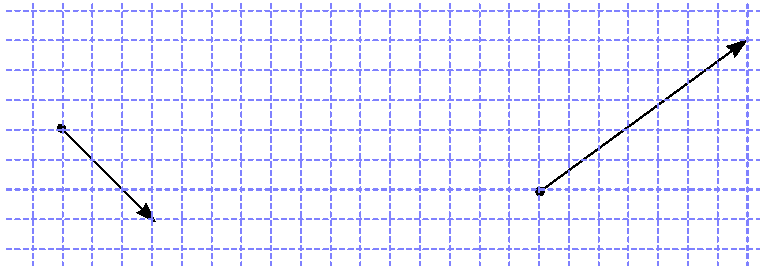
\includegraphics[width=0.65\textwidth]{lxxts-kiirused_.pdf}
\end{center}

\newpage
\yl{LAEVA VETTELASKMINE}
Laeva lastakse aeglaselt mööda kaldpinda vette. Selleks, et laev liiga kiiresti ei libiseks, hoitakse seda paigal laeva ninasse kinnitatud tugeva köie abil (vt joonist). Laeva mass on $m$,  kaldpinna kaldenurk horisondi suhtes on $\alpha$ ning hõõrdetegur laeva ja kaldpinna vahel on $\mu$. Leidke laeva paigalhoidmiseks vajalik minimaalne tõmbejõud $T_{min}=|\overrightarrow{T}_{min}|$ köies. Eeldage, et laev veel vett ei puuduta.
\punktid{12} \autor{Päivo Simson}
\begin{center}
	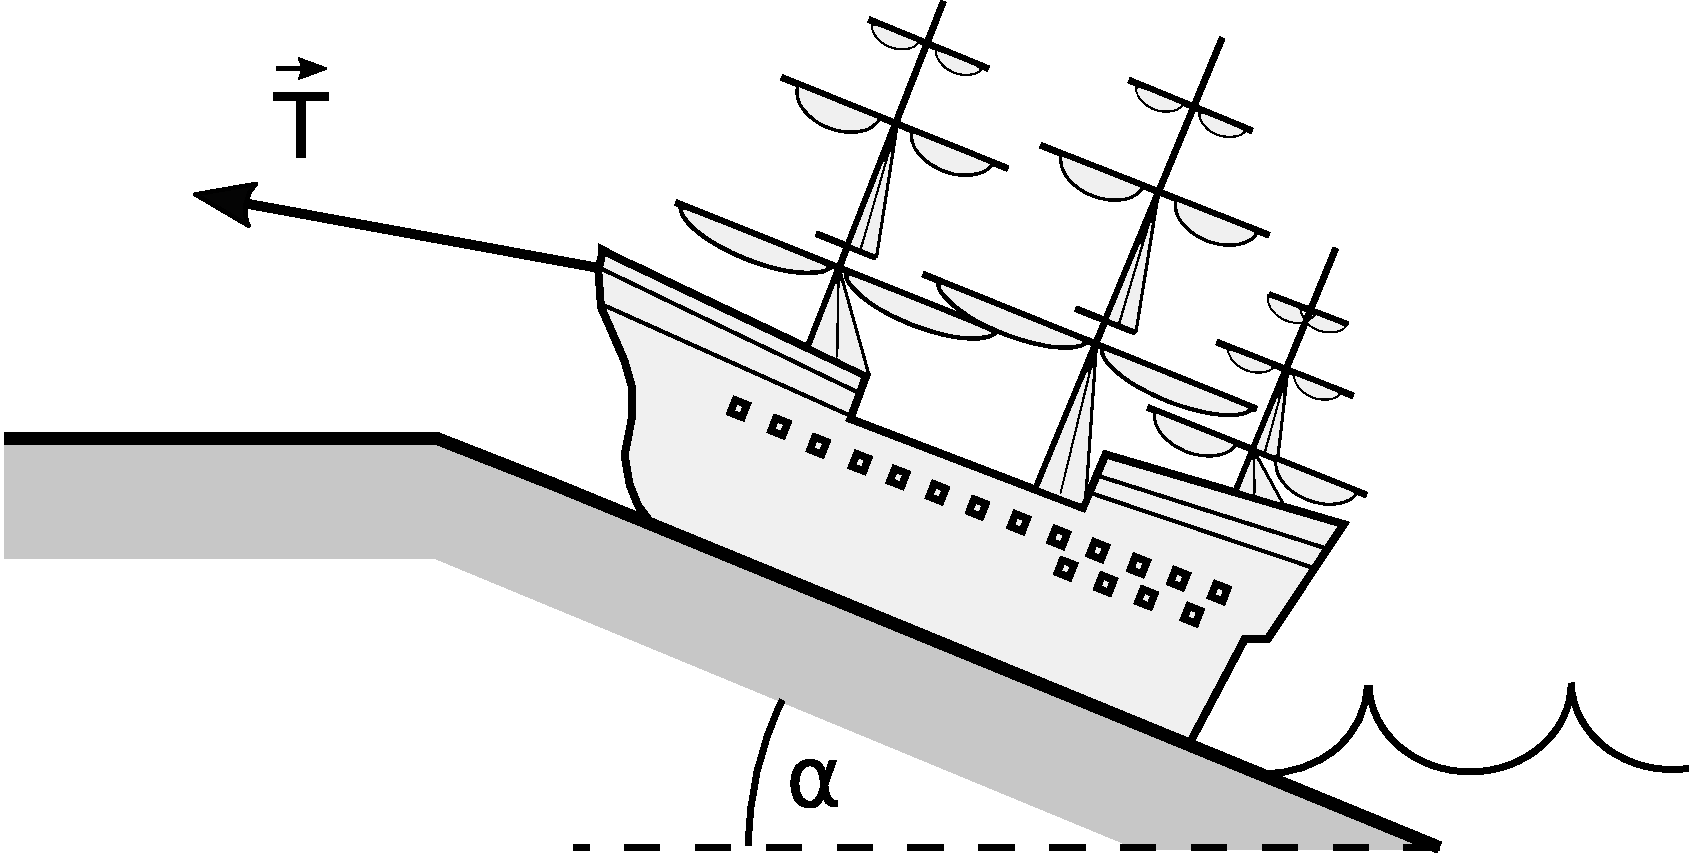
\includegraphics[width=0.4\linewidth]{laev_03.pdf}
\end{center}

\end{document}
